
\section{Methodology} \label{sec:hMethods}

% \subsection{Swept time-space decomposition}

The swept rule exhausts the domain of dependence---the portion of the space-time grid that can be solved given a set of initial values, referred to here as a ``block''---before passing the grid points on the borders of each process.
We refer to the program that implements the swept rule as \texttt{Swept}, and the program that uses naive domain decomposition, that is passing between processes at each timestep, is referred to as \texttt{Classic}.
This way the simulation may continue until no spatial points have available stencils; the required values may then be passed to the neighboring process (i.e., neighboring subdomain) in a single communication event.
Both Alhubail and Wang, and Magee and Niemeyer, provide detailed explanations and graphical depictions
of the swept rule in one dimension, for various architectures~\cite{alhubail:16jcp, OurJCP}.

The heterogeneous one-dimensional swept rule begins by partitioning the computational grid and
allocating space for the working array in each process.
In this case, the working array is of type \texttt{states}, a plain old data C struct that contains the
dependent and intermediate variables needed to continue the procedure from any time step.
Working array size is determined by the number of domains of dependence controlled by the process,
$nBlocks$, and the number of spatial points covered by a domain of dependence, $tpb$ (threads per block).
Here we use ``block'' to represent a domain of dependence; it comes from the GPU\slash CUDA
construct representing a collection of threads.
The program allocates space for $nBlocks \times tpb + (tpb+2)/2$ spatial points and initializes the
first $nBlocks \times tpb + 2$ points.
The initialized points require two extra slots so the edge domains
can build a full domain width on their first step.
Interior domains in the process share their edges with their neighbors; there is no risk of
race conditions since even the simplest numerical scheme requires at least two values in the
\texttt{state} struct, which allows the procedure to alternate reading and writing those values.
Therefore, even as a domain writes on an edge data point that its neighbor must read,
the value the neighbor requires is not modified.

The first cycle completes when each domain has progressed to the sub-time step $tpb/2$
where it has computed two values at the center of the spatial domain.
At this point each process passes the first $tpb/2 + 1$ values in its array to the left neighboring process.
Each process receives the neighbor's buffer and places it in the last $tpb/2 + 1$ slots; that is, starting at the $nBlocks \times tpb$ index.
It proceeds by performing the same computation on the centerpoints, starting at global index $tpb-1$ (adjusted index $tpb/2-1$), of the new array and filling in the uncomputed grid points at successive sub-time steps with a widening spatial window until it reaches a sub-time step that has not been explored at any spatial point and proceeds with a contracting window.
Geometrically, the first cycle completes a triangle, the second completes a diamond.
When the diamond is complete, it passes the last $tpb/2 + 1$ time steps in the array and inputs the received buffer starting at position 0.
Now it performs the diamond procedure again, this time the global and adjusted index are identical and it starts at index $tpb/2 - 1$.

The procedure continues in this fashion until the final time step is reached, at which point it stops after the expanding window reaches the domain width and outputs the solution which is now current at the same time step within and across all domains and processes.
Therefore, the triangle functions are only used twice if no intermediate time step results are output, the rest of the cycles are completed in a diamond shape.

% \section{Implementation} \label{sec:hImplement}

\subsection{Primary data structure} \label{sec:hPrimaryData}

Implementing the swept rule for problems amenable to single-step PDE schemes is straightforward,
but dealing with more realistic problems often requires more complex, often multi-step numerical schemes.
Managing the working array and developing a common interface for these schemes, requires making design decisions that have substantial impacts on performance.

One strategy for dealing with this complexity we term \texttt{flattening} since it flattens the
domain of dependence in the time dimension by combining several potential atomic stages into
single steps with wider stencils. This strategy is more memory efficient for the working array which contains instances of the primary data structure at each spatial point,
but it cannot easily accommodate different methods and equations.
It also introduces additional complexity from parsing the arrays and requires additional register memory
for function and kernel arguments and ancillary variables.


In the new implementation shown here we use the \texttt{lengthening} strategy, also referred to as ``atomic decomposition'', which is instantiated as a struct to generalize the stages into a user-defined data type.
It requires more memory to be used in the primary data structure; for instance, our \texttt{flattening} version
of the Euler equations carried six doubles per spatial point since the pressure ratio used by the
limiter was rolled into the flattened step.
These strategies are described in Figures~\ref{f:Longpseudo} and ~\ref{f:flatPseudo}.
By restricting the stencil to three points, the \texttt{lengthening} method requires the pressure ratio
to be stored and passed through the memory hierarchy meaning the data structure carries seven doubles per spatial point for the Euler equation.

\begin{figure}[bt]
    \begin{minipage}[t]{0.48\textwidth}
        \begin{lstlisting}
        // Q = {rho, rho*u, rho*E}
        struct states {
            double3 Q[2]; // State Variables
            double Pr; // Pressure ratio
        };

        __device__ __host__
        void stepUpdate(states *state, const int idx, const int tstep)
        {
            int ts = tstep % 4; // 4 is number of steps in cycle
            if (tstep & 1)  pressureRatio(state, idx, ts);
            else            eulerStep(state, idx, ts);
        }

        __global__ void classicStep(states *state, const int tstep)
        {
            int gid = blockDim.x * blockIdx.x + threadIdx.x + 1;
            stepUpdate(state, gid, tstep);
        }
        \end{lstlisting}
        \caption{Skeleton for the \texttt{lengthening} method in the \texttt{Classic} program. The \texttt{states} structure contains all the information to step forward at any point.  The user is only responsible for writing the \texttt{eulerStep} and \texttt{pressureRatio} functions and accessing the correct members based on the timestep count}
        \label{f:Longpseudo}
    \end{minipage}
    ~
    \begin{minipage}[t]{0.48\textwidth}
        \begin{lstlisting}
        __global__ void classicStep(const double *s_in, double *s_out, bool final)
        {
        int gid = blockDim.x * blockIdx.x + threadIdx.x;
        //number of spatial points - 1
        int lastidx = ((blockDim.x*gridDim.x));
        int gids[5];

        for (int k = -2; k<3; k++) gids[k+2] = (gid + k) % lastidx;

        //Final is false for predictor step, true otherwise.
        if (final) s_out[gid] += finalStep(s_in, gids);
        else       s_out[gid]  = predictorStep(s_in, gids);
        }
        \end{lstlisting}
        \caption{Skeleton for the \texttt{flattening} method in the \texttt{Classic} program. The sub-timesteps are compressed to a step with a wider stencil. The two arrays which alternate reading and writing are explicitly passed and traded in the calling function.}
        \label{f:flatPseudo}
    \end{minipage}
\end{figure}

To gauge the influence of this change in primary data structure, we compared the performance of
the Kuramoto--Sivashinksy (KS) equation, using a second-order
Runge--Kutta finite-difference method in time and central differencing in space with
periodic boundary and initial conditions.
A complete explanation of this method applied to the KS equation can be found in the appendix of our previous paper~\cite{OurJCP}.
We implemented each combination of the classic and swept decomposition techniques and the \texttt{flattening}
and \texttt{lengthening} data structures.
We used the KS equation because it was easy to adapt to both styles due to its periodic boundary conditions,
and since it requires four atomic stages in the lengthened structure such that the versions are suitably different.

\begin{figure}[htbp]
    \centering
    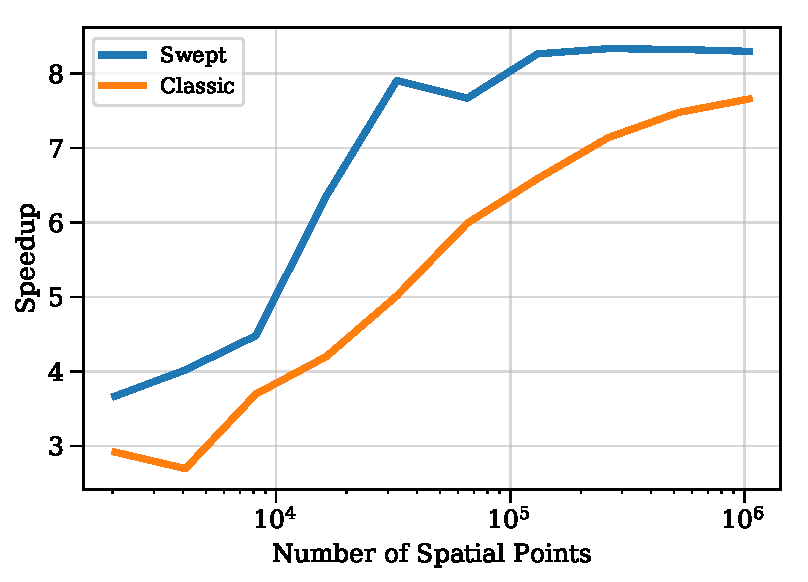
\includegraphics[width=.7\textwidth]{SpeedupcArray}
    \caption{Speedup of \texttt{flattening} compared to the same scheme using \texttt{lengthening} applied to the KS equation on the GPU only.}
    \label{f:lflat}
\end{figure}

Figure~\ref{f:lflat} compares the performance of the memory storage techniques in an
experiment executed on a workstation with an \WCPU{} and an \WGPU{}.
The \texttt{Classic} program using the \texttt{flattening} method using is compared to the same program using the \texttt{lengthening} method and likewise for \texttt{Swept}.
As Figure~\ref{f:lflat} shows, the \texttt{flattening} method is faster than \texttt{lengthening} for both decomposition methods and gets faster as the number of spatial points increases.
There is not much difference in the trends between swept and classic decomposition methods, but it does appear that the less performative data structure affects the \texttt{Swept} program more.
Much of the reason that \texttt{lengthening} is substantially less performative
is an artifact of GPU architecture, so it is difficult to generalize the results of this study to
heterogeneous systems. GPU memory accesses, from global and shared memory, are more sensitive to
irregularities because of the parallel nature of the device as a whole; it is not designed to be used serially.
The extra memory requirements of the \texttt{lengthening} method also consume limited shared memory
resources on the GPU, which diminishes the L1 cache capacity used to accelerate global memory accesses
on Kepler-generation GPUs.
While locality is a significant issue for effective CPU memory accesses, it has a larger impact on GPU performance.

We feel that it is important to present these findings so that others who implement the swept rule will
have a more thorough understanding of the tradeoffs inherent in the program design choices across architectures.
But, since the \texttt{Swept} and \texttt{Classic} algorithms perform similarly compared to the
\texttt{flattening} method, the conclusions we derive from our experiments using the \texttt{lengthening}
method remain valid.
And we believe that, in this case, the values that the \texttt{lengthening} method provides:
extensibility and regularity are of greater value than the absolute best performance.

\subsection{Program design features}

Our earlier implementation of the swept rule for GPUs~\cite{OurJCP} required creating separate single-file
\CC{}\slash CUDA programs for each problem.
We have determined that this approach is insufficient for enabling the support for further exploration that is essential to the accurate analysis of highly architecture
and problem dependent algorithms.
Our previous analysis showed that the performance characteristics of the GPU-based swept rule depend
on the boundary conditions, numerical method, and governing equation(s).
In this work we endeavor to create a convenient and reusable interface through which other can reproduce our experiments, explore different equations and numerical methods to examine performance characteristics the performance characteristics of the swept rule.

We have created this interface by separating the domain decomposition and grid generation, and passing
a map between the equation-specific part of the code, defined by the user, and the generic part of the code.
In practice, the user defines an initialization procedure that defines any constant terms in the
governing equation(s), e.g., the Fourier number in the heat equation.
The user is guaranteed to receive the standard grid variables, e.g., $\Delta x$, $\Delta t$, in the map
along with any other values needed to define the constant terms, i.e., the thermal diffusivity
for the heat equation.
The user defines these non-standard constant terms in a JSON file passed to the program on the command line
or as command line key/value pair arguments. By defining these fundamental concepts in a separate JSON
file, variables that define the grid or material constants in the equations can be redefined without
the need to recompile.

This structure requires a solver interface that operates on every equation and numerical scheme
the same way, which in turn requires the use of a different strategy for decomposing more complex
equations and domains.
The clearest way to create a general form for a user-defined equation is to oblige the user to decompose
the numerical formula into atomic stages, a series of steps requiring only three-point stencils as described
by Wang~\cite{WangDecomp}, and provide a step counter in the root function to define the sequence of stages.
The user must also define the data structure where results of each stage are collected, this structure takes the form of a plain old data struct named \texttt{states}.

Our first study showed that shared memory is the most effective means of exploiting the memory hierarchy
for this application on this generation of GPUs~\cite{OurJCP}.
We rely on this conclusion here to again use the GPU characteristics to determine the size of the
domains of dependence.
Each GPU thread is mapped to a single spatial point and each CPU process, having only one available thread,
traverses a number of domains in serial.
This limits the size of the domain of dependence to the allowable number of threads in each block launched
in the GPU kernel, which depends on the occupancy of the most-restrictive kernel as determined by the shared
memory and register resource requirements.


Our approach organizes the available processors by assigning each GPU on a node to one
MPI process (i.e., CPU core) on the same node that has exclusive control over it; that process also
manages one domain on either side of the GPU subdomain.
Thus, to facilitate this, each MPI process comprises a positive, even number of subdomains.
All subdomains on a node must contain the same number of points, and all MPI processes evaluate the
same number of subdomains.
Processes that control a GPU simply ``contain'' additional subdomains equal to the GPU affinity times
the number of domains assigned to an MPI process.
For example, a domain of 160 points could be decomposed into subdomains of 16 points on a node with
four CPU cores and one GPU; each processor would compute the time-stepping for two subdomains, while the
MPI process controlling the GPU comprises four subdomains in total (two on the CPU, and two on the GPU).
This corresponds to a GPU affinity of one, since the GPU subdomain equals the CPU subdomain sizes.

Assigning a GPU to a single process reduces complexity and avoids using the GPU at the spatial
boundaries where imposing boundary conditions causes thread divergence.
This is useful from a conceptual standpoint, even though we previously found that boundary
conditions only affect GPU performance in a minor way~\cite{OurJCP}.

Our program uses the MPI\allowbreak+CUDA paradigm, and assigns one MPI process to each core for the life of a program.
We considered using an MPI\allowbreak+OMP\allowbreak+CUDA paradigm by assigning an MPI process to each socket, and
launching threads from each process to occupy the individual cores, but recent work has shown that
this approach rarely improves performance on clusters of limited size for finite volume or finite
difference solvers~\cite{IDAHO_MPI_CUDA, PerfAnalysisHetero}.
This conclusion has led widely used libraries, such as PETSc, to opt against a paradigm of threading
within processes~\cite{MillsPetsc}.


\subsection{Experimental method} \label{sec:ExpMethod}

We endeavor to address the questions presented in Section~\ref{sec:obj1} by varying
three primary attributes of the decomposition: threads per block, GPU affinity, and grid size.
We repeatedly executed our two test equations, the heat and Euler equations, over the
experimental domain of these variables using \texttt{Swept} and \texttt{Classic}, exchanging borders every
sub-time step, decomposition methods.
In our program implementing the swept rule in one-dimension on heterogeneous systems, hSweep,
threads per block is synonymous with the size of the domain-of-dependence, but we refer to it using GPU terminology because each domain is launched as a block of threads on the GPU.
A block is an abstract grouping of threads that share an execution setting, a streaming multiprocessor, and access to a shared memory space, a portion of the GPU L1 cache.
hSweep uses the swept rule to avoid communication between devices and processes and exploits the
GPU memory hierarchy to operate on shared memory quantities closer to the processor.
Since this multi-level memory scheme influences the swept-rule performance and GPU execution, the resultant effects are difficult to predict.
The independent variables GPU affinity and grid size are more straightforward.
The grid size is the total number of spatial points in the simulation domain, and is provided
by the user; however, the program revises this number to provide a grid that fits the other program settings
that the grid must accommodate: the threads per block, GPU affinity, and number of processes.
The GPU affinity is the portion of the computational grid that is processed by the GPU,
expressed as a ratio of the number of domains-of-dependence assigned to the GPU to those assigned to a single MPI process (on a CPU core).
GPU affinity, like the other experimental variables, should be given as an integer, since we have
determined that it is beneficial for the GPU to handle a larger portion of the overall grid
than a single MPI process.

In our previous study of the swept rule~\cite{OurJCP}, the experimental domain was clearly
defined by the particular properties of GPU architecture.
Because a warp contains 32 threads and a block cannot exceed 1024 threads, here we constrained
the number of threads per block, which is also the width of the domain of dependence, in our experiments
to be a power of 2 from \numrange{32}{1024}.
To enforce regularity, we constrained our experimental problem size---the number of spatial points in the
grid---to be a power of 2 larger between \num{1024} and $2^{21}$.

Using CPU parallelism across 40 processes and GPU affinity as a variable of interest in this study, eliminates the potential for regularity in the experimental grid.
To remedy this, we relaxed the constraints on the experimental launch conditions so that the number of
threads per block is required to be a multiple of 32 from \numrange{32}{1024} rather than a power of two.
In addition, at runtime the program uses the number of processes, threads per block, GPU affinity,
and desired grid size to determine the closest grid size to the requested value that accommodates the constraints.
This results in different grid sizes for the same experimental settings.
To assess the performance at various settings, we interpolated each result to the requested grid size
from the actual grid size.

The addition of GPU affinity as an independent variable introduces further complication to the experimental domain.
While our experiments are constrained by GPU architecture in threads per block and by the number
of processes and blocks in problem size, we initially have no clear indication of what the
experimental limits of GPU affinity should be---so we took an iterative approach.
First, we ran a screening study and executed the programs over a broad range of conditions:
eight block sizes from \numrange{64}{768}, 11 GPU affinities from \numrange{0}{80}, and
four grid sizes from \numrange{5e5}{e7}.
This showed us that the best affinity for all the programs would likely fall between \numrange{20}{60}
and that all threads per block values could provide the best performance.
This was somewhat disappointing, since we had hoped to narrow the range for both GPU affinity and
threads per block further in order to experiment on a finer increment of grid size in a reasonable amount of time.
For the final experiment, we used the same block sizes, GPU affinity values from \numrange{20}{60}
in increments of 4, and seven grid sizes over the same range.

In this study, we solve the one-dimensional heat equation using a first-order forward in time, central in space
method and Euler equations for a shock wave using a second-order finite-volume scheme with minmod limiter.
Explanations of these methods can be found in the appendix of our previous paper~\cite{OurJCP}.
